\chapter{EXPERIMENTAL RESULTS}
\label{chap-four}

\section{Experimental Results}

This chapter presents the data from the experiment discussed in Chapter \ref{chap-three}.

\section{Base Data}
Readings in the impedance tube with no acoustic absorption material present are shown in this section.

% Absorption Coefficient - Empty
\begin{figure}[hbtp]
    \centering
    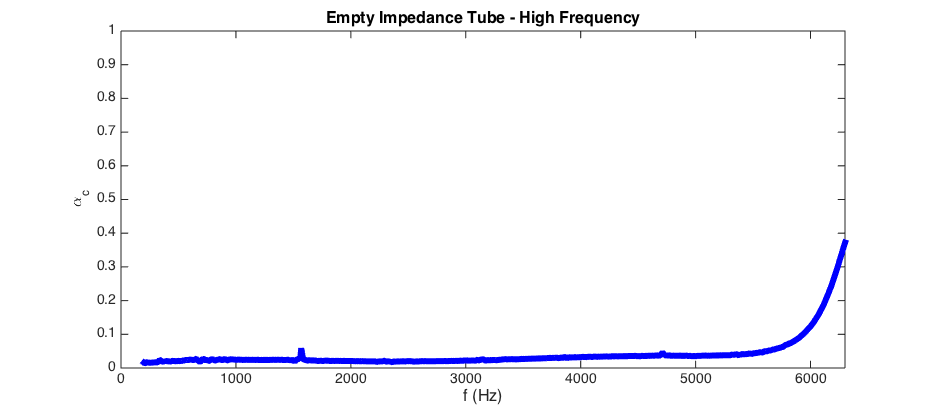
\includegraphics[width=1\textwidth]{Chapter-4/figs/Afigempty}
    \caption{Absorption Coefficient vs. Frequency - Empty Tube}
    \label{fig:Afigempty}
\end{figure}

Figure \ref{fig:Afigempty} shows the base values for absorption coefficient that the impedance tube system reads with no sample present.

% Absorption Coefficient - O Ring
\begin{figure}[hbtp]
    \centering
    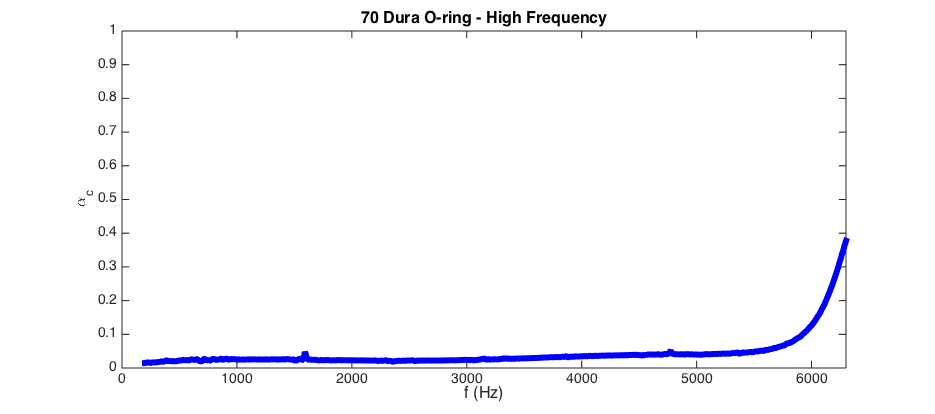
\includegraphics[width=1\textwidth]{Chapter-4/figs/AfigOring}
    \caption{Absorption Coefficient vs. Frequency - 70-Dura Oring}
    \label{fig:AfigOring}
\end{figure}
\clearpage
Figure \ref{fig:AfigOring} shows how adding the O-ring material has little influence in the data recorded by the system.

% Figures
\section{Commercial Materials}
Commercial material data is shown in this section.

\subsection{Foam Materials}
% Absorption Coefficient - BK Foam
\begin{figure}[hbtp]
    \centering
    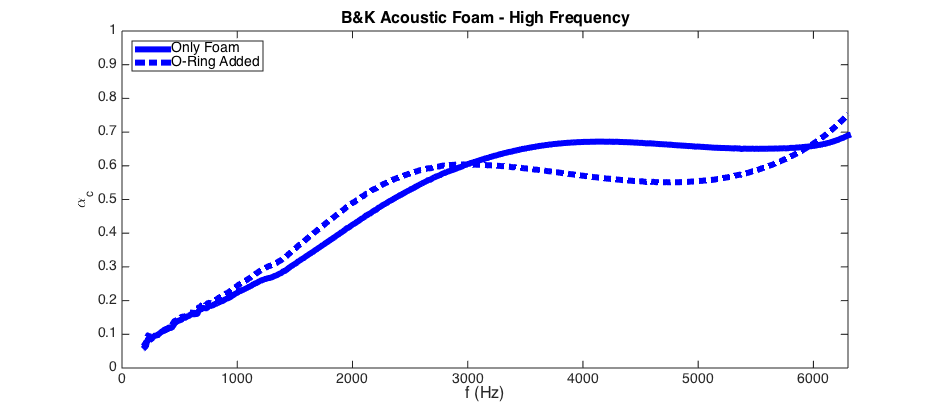
\includegraphics[width=1\textwidth]{Chapter-4/figs/AfigBKfoam}
    \caption{Absorption Coefficient vs. Frequency - B and K Foam}
    \label{fig:AfigBKfoam}
\end{figure}

% Absorption Coefficient - Auralex Foam
\begin{figure}[hbtp]
    \centering
    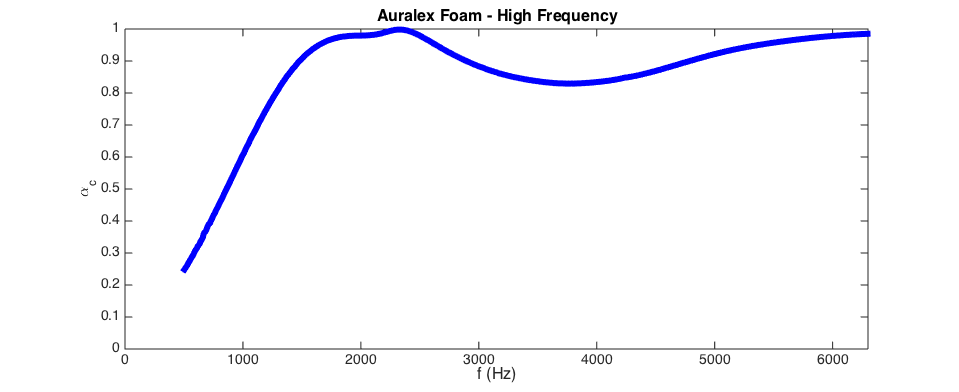
\includegraphics[width=1\textwidth]{Chapter-4/figs/AuralexFoam}
    \caption{Absorption Coefficient vs. Frequency - Auralex Foam}
    \label{fig:AuralexFoam}
\end{figure}
\clearpage

Figure \ref{fig:AfigBKfoam} and \ref{fig:AuralexFoam} show the results of the tests run for acoustic foams.

\subsection{Fiberglass}
% Absorption Coefficient - EX15-3 Fiberglass
\begin{figure}[hbtp]
    \centering
    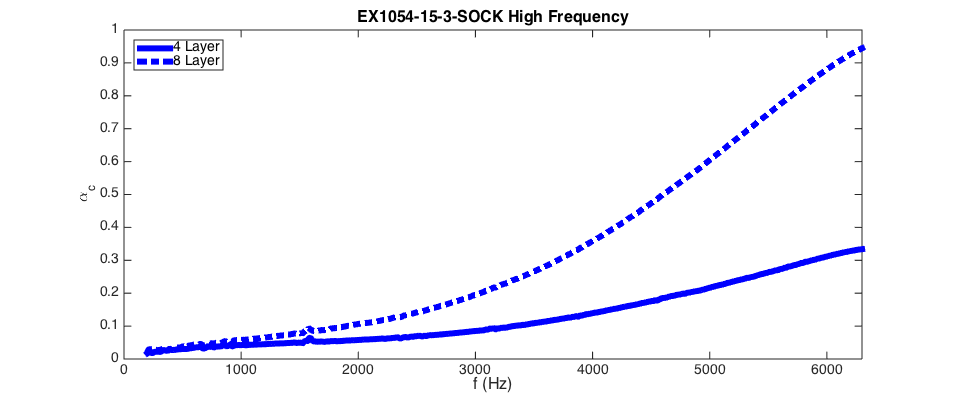
\includegraphics[width=1\textwidth]{Chapter-4/figs/AfigSOCK15-3}
    \caption{Absorption Coefficient vs. Frequency - EX1054-15-2 - Fiberglass}
    \label{fig:AfigSOCK15-3}
\end{figure}

% Absorption Coefficient - Raw Fiberglass (Thick - 2")
\begin{figure}[hbtp]
    \centering
    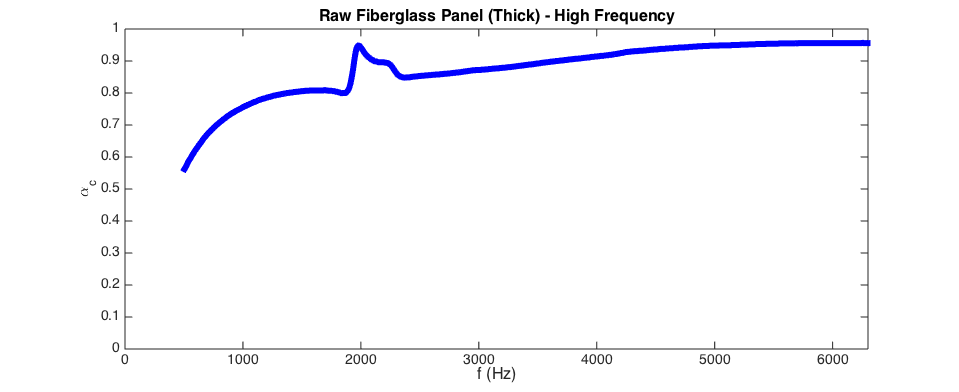
\includegraphics[width=1\textwidth]{Chapter-4/figs/RawFiberglassThick}
    \caption{Absorption Coefficient vs. Frequency - Raw Fiberglass (2" Thick)}
    \label{fig:RawFiberglassThick}
\end{figure}

% Absorption Coefficient - Raw Fiberglass (Thin - 1")
\begin{figure}[hbtp]
    \centering
    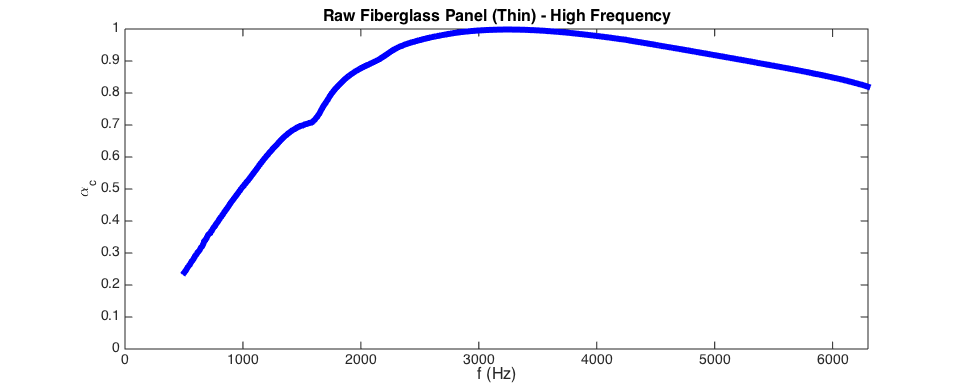
\includegraphics[width=1\textwidth]{Chapter-4/figs/RawFiberglassThin}
    \caption{Absorption Coefficient vs. Frequency - Raw Fiberglass (1" Thick)}
    \label{fig:RawFiberglassThin}
\end{figure}
\clearpage

Figure \ref{fig:AfigSOCK15-3} is a Sock type Fiberglass material, while figures \ref{fig:RawFiberglassThick} and \ref{fig:RawFiberglassThin} show a Fiberglass panel material in two thickness; 2" and 1" respectively.

\subsection{Polymer Materials}
% Absorption Coefficient - EX15-1 nylon
\begin{figure}[hbtp]
    \centering
    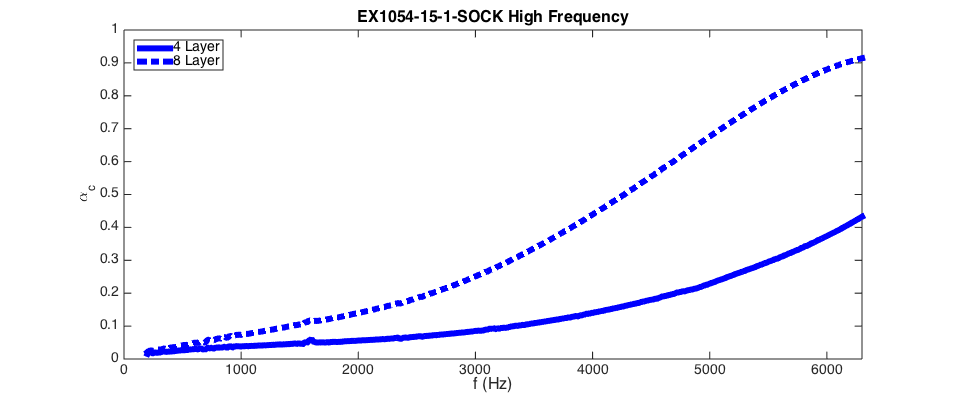
\includegraphics[width=1\textwidth]{Chapter-4/figs/AfigSOCK15-1}
    \caption{Absorption Coefficient vs. Frequency - EX1054-15-1 - Nylon}
    \label{fig:AfigSOCK15-1}
\end{figure}

% Absorption Coefficient - EX15-2 PET
\begin{figure}[hbtp]
    \centering
    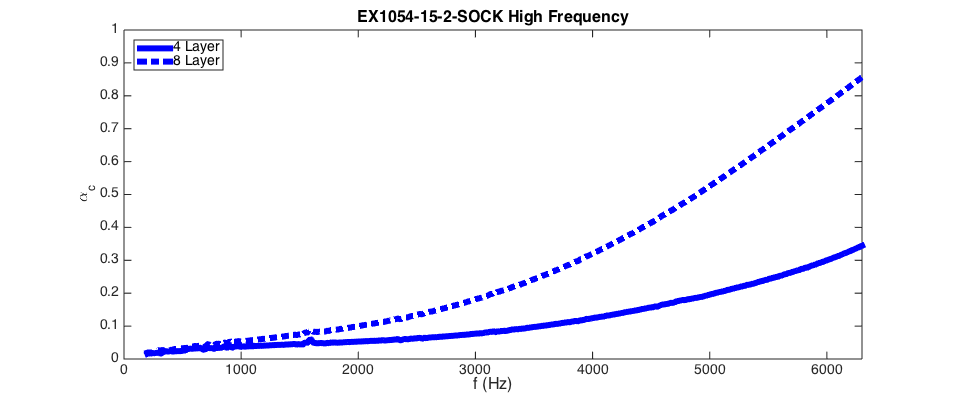
\includegraphics[width=1\textwidth]{Chapter-4/figs/AfigSOCK15-2}
    \caption{Absorption Coefficient vs. Frequency - EX1054-15-2 - PET}
    \label{fig:AfigSOCK15-2}
\end{figure}

% Absorption Coefficient - Auralex Cotton
\begin{figure}[hbtp]
    \centering
    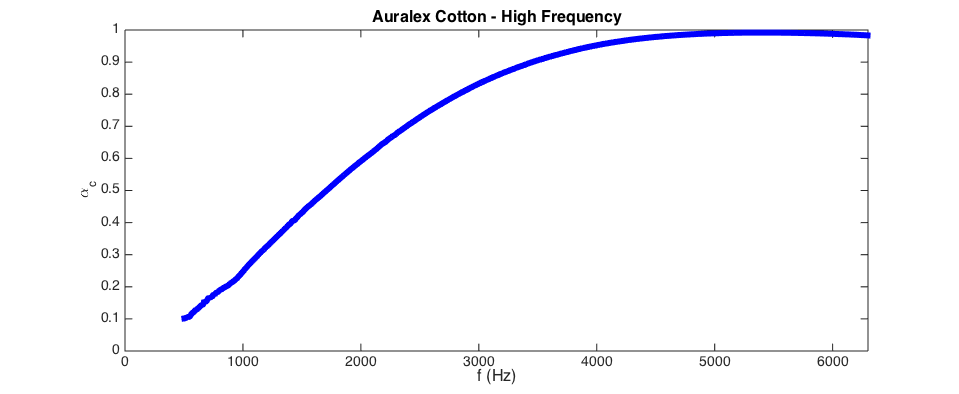
\includegraphics[width=1\textwidth]{Chapter-4/figs/AuralexCotton}
    \caption{Absorption Coefficient vs. Frequency - Auralex Cotton}
    \label{fig:AuralexCotton}
\end{figure}

% Absorption Coefficient - Auralex Compressed Polyester
\begin{figure}[hbtp]
    \centering
    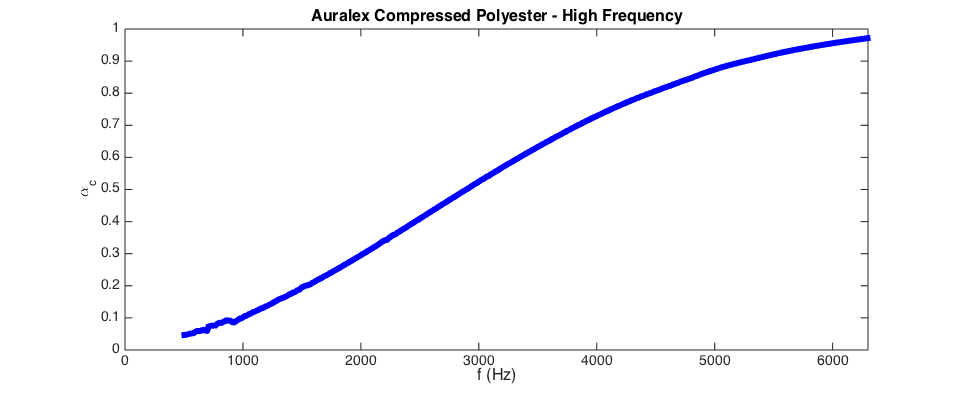
\includegraphics[width=1\textwidth]{Chapter-4/figs/AuralexCompPoly}
    \caption{Absorption Coefficient vs. Frequency - Auralex Compressed Polyester}
    \label{fig:AuralexCompPoly}
\end{figure}

Figures \ref{fig:AfigSOCK15-1}, and \ref{fig:AfigSOCK15-2} show sock materials of Nylon and PET respectively. Figure \ref{fig:AuralexCotton} shows compressed cotton from Auralex, and Figure \ref{fig:AuralexCompPoly} shows compressed polyester from Auralex.

\clearpage

\section{Cellulose Acetate Materials}
This section shows data for the Cellulose Acetate material tests.

% Absorption Coefficient - Raw Tow
\begin{figure}[hbtp]
    \centering
    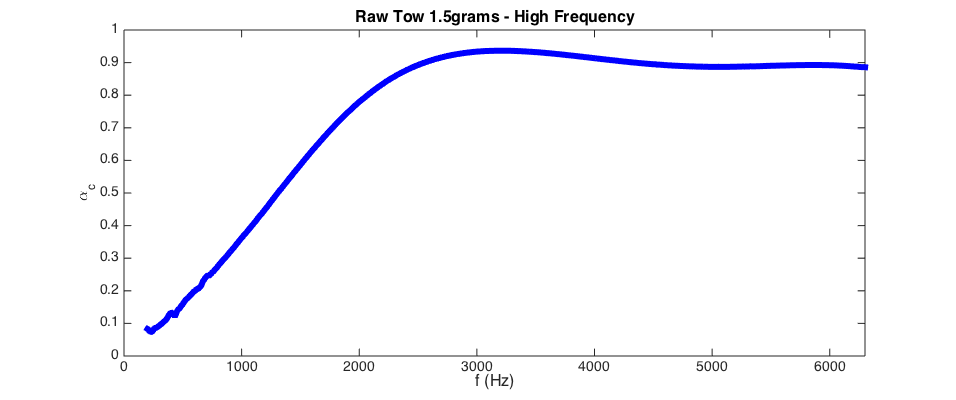
\includegraphics[width=1\textwidth]{Chapter-4/figs/Afigrawtow}
    \caption{Absorption Coefficient vs. Frequency - Raw Tow}
    \label{fig:Afigrawtow}
\end{figure}

Figure \ref{fig:Afigrawtow} shows the results from raw tow of $1.5$ grams.

\subsection{Sock Materials}
Cellulose Acetate Sock materials are presented below. They are divided into two sections for clarity: high and low denier respectively.
\clearpage

\subsubsection{High Denier Materials}
% Absorption Coefficient - EX8-2
\begin{figure}[hbtp]
    \centering
    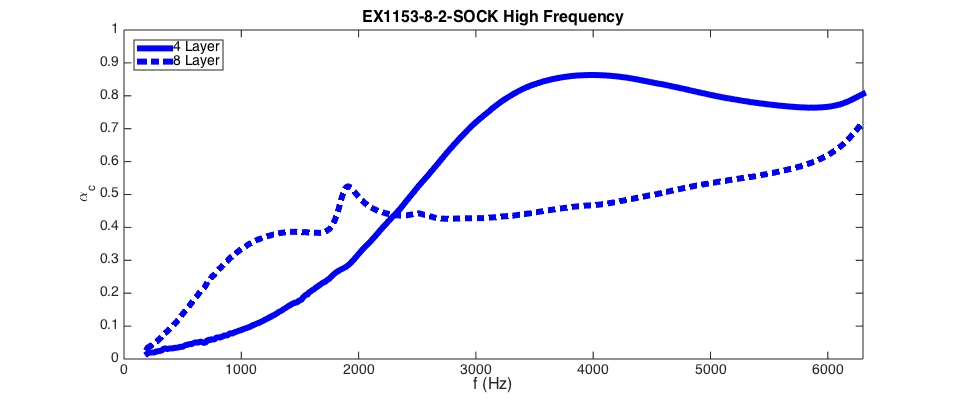
\includegraphics[width=1\textwidth]{Chapter-4/figs/AfigSOCK8-2}
    \caption{Absorption Coefficient vs. Frequency - EX1154-8-2}
    \label{fig:AfigSOCK8-2}
\end{figure}

% Absorption Coefficient - EX9-5
\begin{figure}[hbtp]
    \centering
    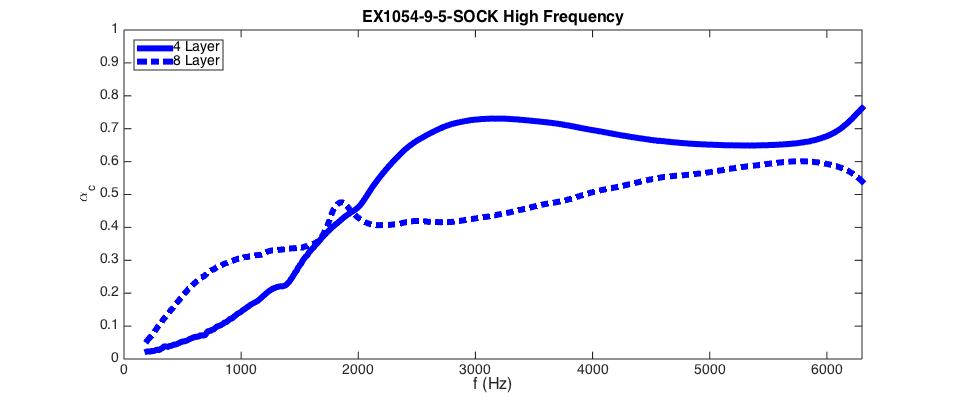
\includegraphics[width=1\textwidth]{Chapter-4/figs/AfigSOCK9-5}
    \caption{Absorption Coefficient vs. Frequency - EX1054-9-5}
    \label{fig:AfigSOCK9-5}
\end{figure}

% Absorption Coefficient - EX9-6
\begin{figure}[hbtp]
    \centering
    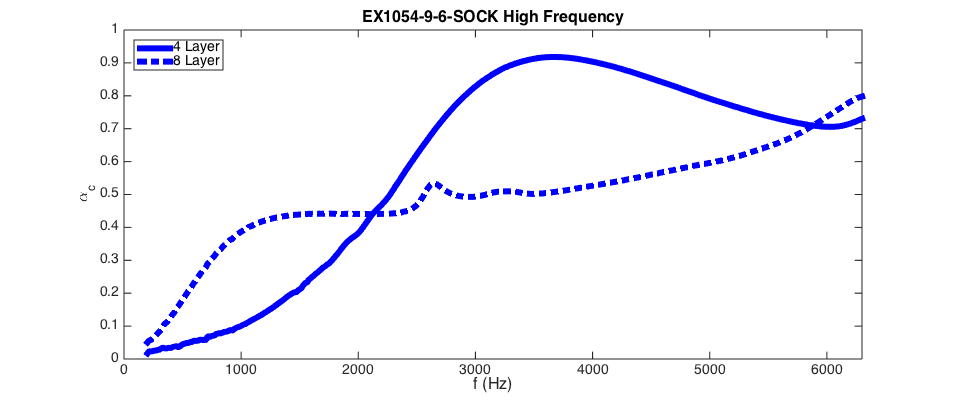
\includegraphics[width=1\textwidth]{Chapter-4/figs/AfigSOCK9-6}
    \caption{Absorption Coefficient vs. Frequency - EX1054-9-6}
    \label{fig:AfigSOCK9-6}
\end{figure}

% Absorption Coefficient - EX18-3
\begin{figure}[hbtp]
    \centering
    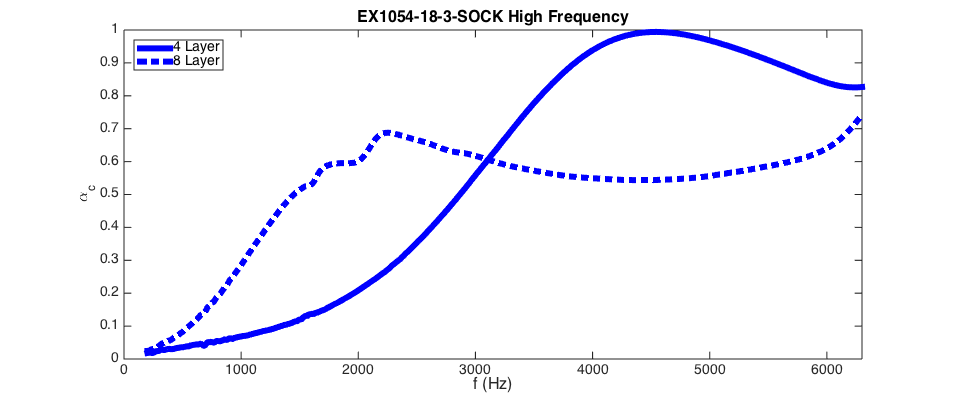
\includegraphics[width=1\textwidth]{Chapter-4/figs/AfigSOCK18-3}
    \caption{Absorption Coefficient vs. Frequency - EX1054-18-3}
    \label{fig:AfigSOCK18-3}
\end{figure}

% Absorption Coefficient - EX18-4
\begin{figure}[hbtp]
    \centering
    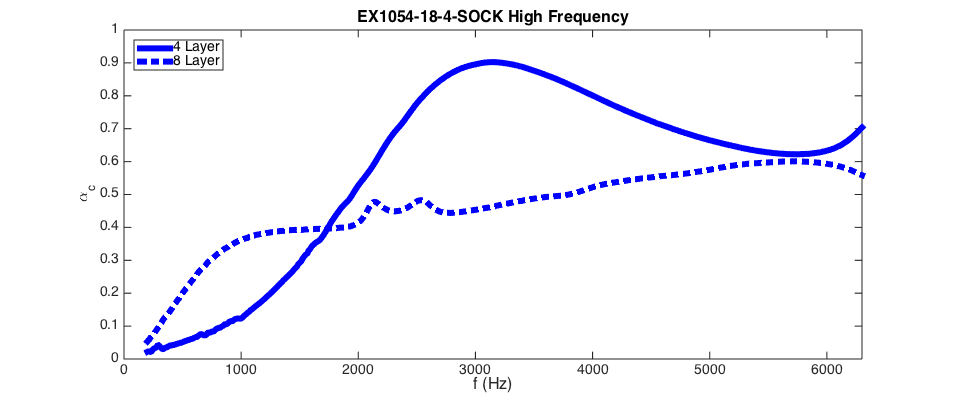
\includegraphics[width=1\textwidth]{Chapter-4/figs/AfigSOCK18-4}
    \caption{Absorption Coefficient vs. Frequency - EX1054-18-4}
    \label{fig:AfigSOCK18-4}
\end{figure}
\clearpage

\subsubsection{Low Denier Materials}

% Absorption Coefficient - EX9-1
\begin{figure}[hbtp]
    \centering
    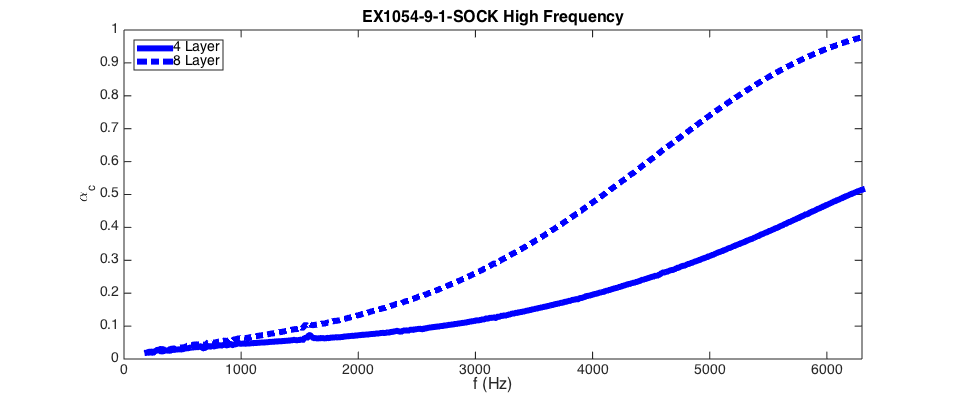
\includegraphics[width=1\textwidth]{Chapter-4/figs/AfigSOCK9-1}
    \caption{Absorption Coefficient vs. Frequency - EX1054-9-1}
    \label{fig:AfigSOCK9-1}
\end{figure}

% Absorption Coefficient - EX9-3
\begin{figure}[hbtp]
    \centering
    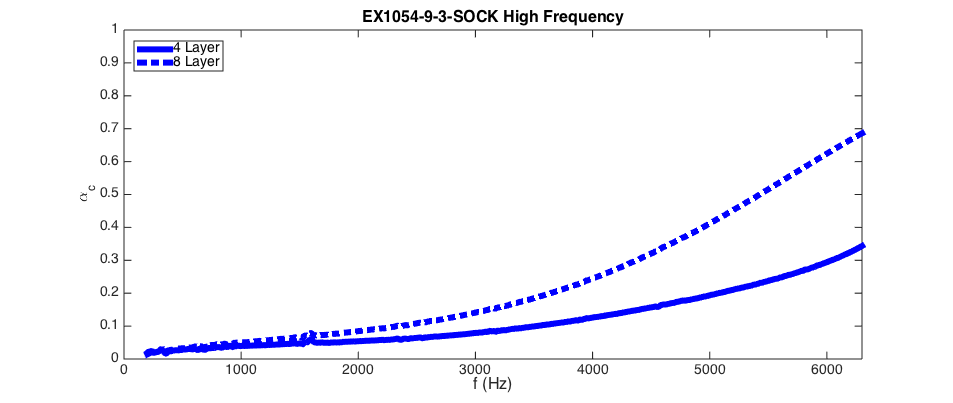
\includegraphics[width=1\textwidth]{Chapter-4/figs/AfigSOCK9-3}
    \caption{Absorption Coefficient vs. Frequency - EX1054-9-3}
    \label{fig:AfigSOCK9-3}
\end{figure}

% Absorption Coefficient - EX9-8
\begin{figure}[hbtp]
    \centering
    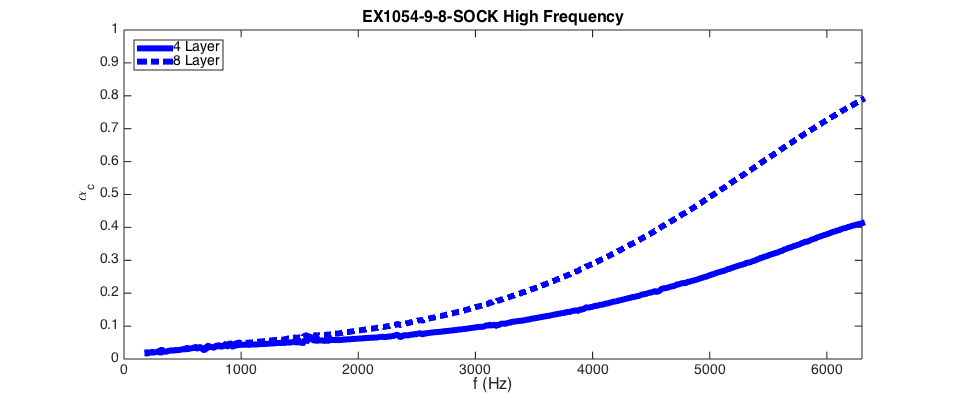
\includegraphics[width=1\textwidth]{Chapter-4/figs/AfigSOCK9-8}
    \caption{Absorption Coefficient vs. Frequency - EX1054-9-8}
    \label{fig:AfigSOCK9-8}
\end{figure}

% Absorption Coefficient - EX9-9
\begin{figure}[hbtp]
    \centering
    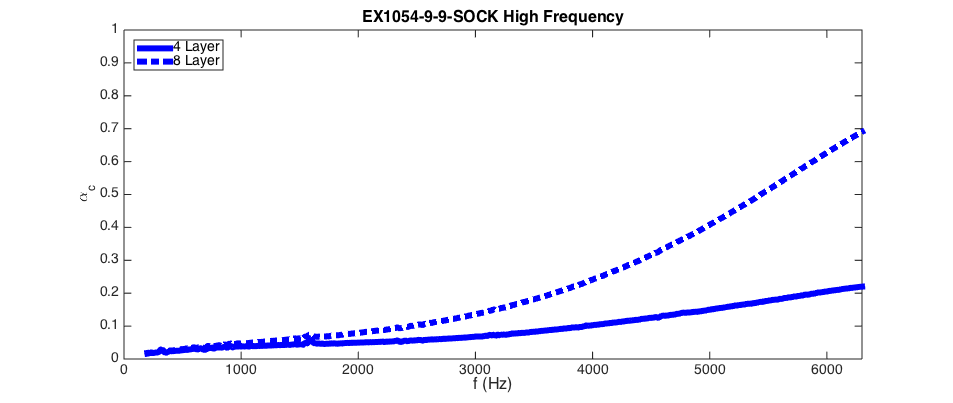
\includegraphics[width=1\textwidth]{Chapter-4/figs/AfigSOCK9-9}
    \caption{Absorption Coefficient vs. Frequency - EX1054-9-9}
    \label{fig:AfigSOCK9-9}
\end{figure}

% Absorption Coefficient - EX18-1
\begin{figure}[hbtp]
    \centering
    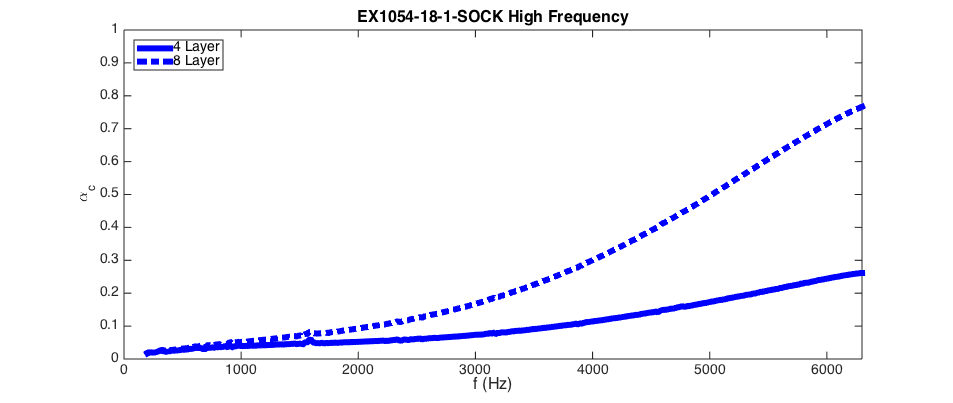
\includegraphics[width=1\textwidth]{Chapter-4/figs/AfigSOCK18-1}
    \caption{Absorption Coefficient vs. Frequency - EX1054-18-1}
    \label{fig:AfigSOCK18-1}
\end{figure}

% Absorption Coefficient - EX18-2
\begin{figure}[hbtp]
    \centering
    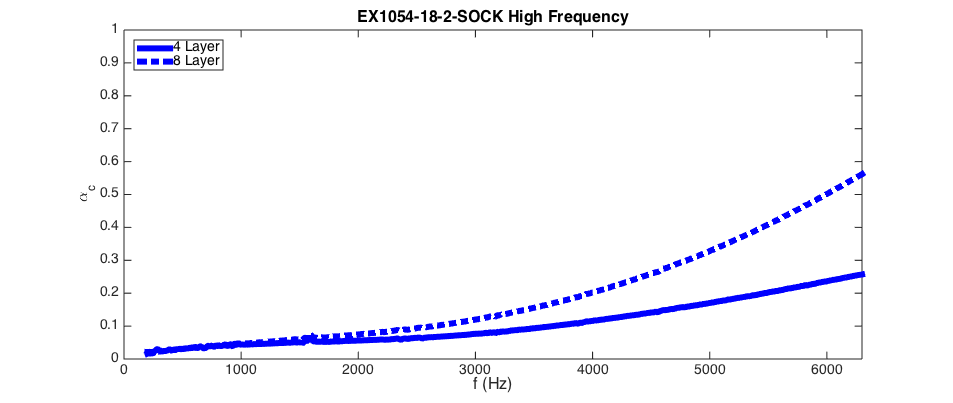
\includegraphics[width=1\textwidth]{Chapter-4/figs/AfigSOCK18-2}
    \caption{Absorption Coefficient vs. Frequency - EX1054-18-2}
    \label{fig:AfigSOCK18-2}
\end{figure}
\clearpage




\subsection{Filter Rod Materials}
Filter Rod test data is presented below.

% Absorption Coefficient - Filter Rod White
\begin{figure}[hbtp]
    \centering
    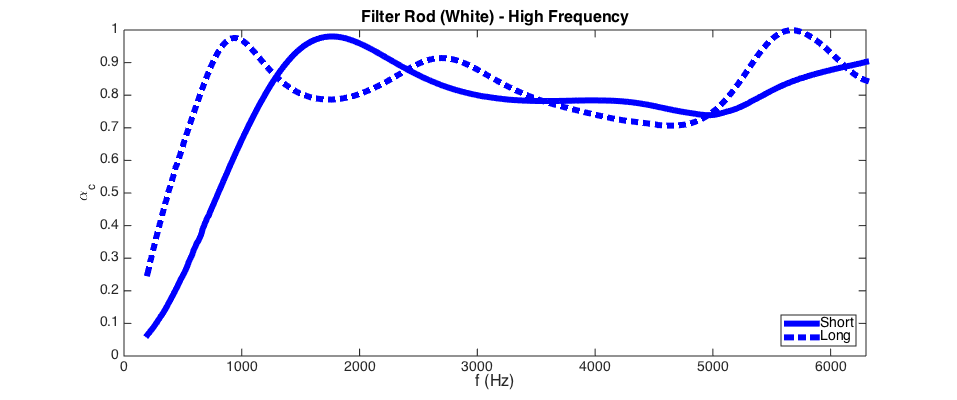
\includegraphics[width=1\textwidth]{Chapter-4/figs/Afigfilterrodwhite}
    \caption{Absorption Coefficient vs. Frequency - White Filter Rod}
    \label{fig:Afigfilterrodwhite}
\end{figure}

% Absorption Coefficient - Filter Rod White no paper
\begin{figure}[hbtp]
    \centering
    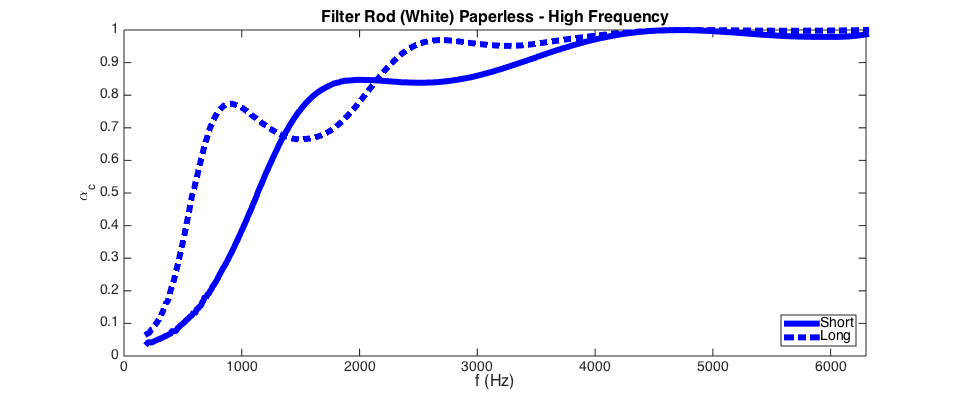
\includegraphics[width=1\textwidth]{Chapter-4/figs/Afigfilterrodwhitenopaper}
    \caption{Absorption Coefficient vs. Frequency - White Filter Rod (no paper)}
    \label{fig:Afigfilterrodwhitenopaper}
\end{figure}

% Absorption Coefficient - Filter Rod Black
\begin{figure}[hbtp]
    \centering
    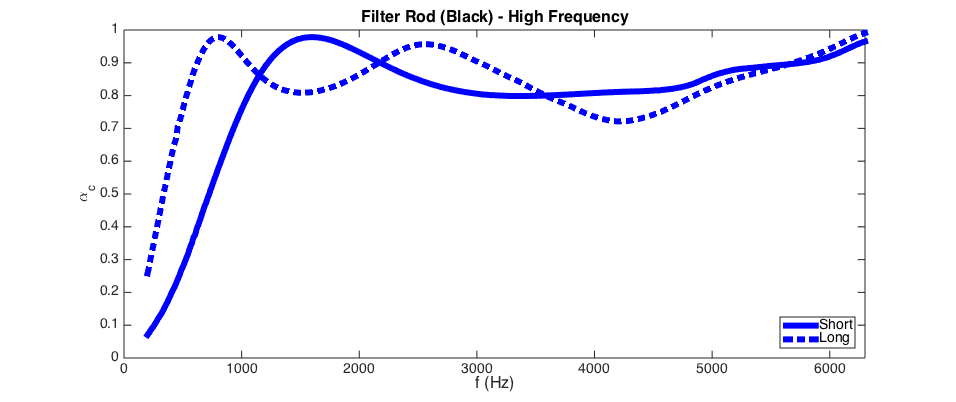
\includegraphics[width=1\textwidth]{Chapter-4/figs/Afigfilterrodblack}
    \caption{Absorption Coefficient vs. Frequency - Black Filter Rod}
    \label{fig:Afigfilterrodblack}
\end{figure}

% Absorption Coefficient - Filter Rod Black no paper
\begin{figure}[hbtp]
    \centering
    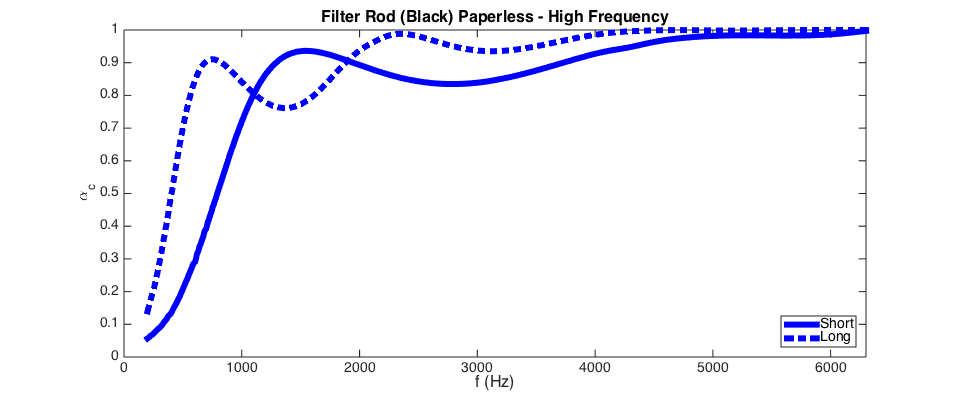
\includegraphics[width=1\textwidth]{Chapter-4/figs/Afigfilterrodblacknopaper}
    \caption{Absorption Coefficient vs. Frequency - Black Filter Rod (no paper)}
    \label{fig:Afigfilterrodblacknopaper}
\end{figure}
\clearpage

\section{Comparing Materials}
After all data has been recorded, trends between data sets start to arise. This section overlays data sets to show similar data. 

\subsection{High Denier vs. Low Denier Mix}
This section compares a sample of relatively high denier with a sample of relatively low denier of equal mass.

% Absorption Coefficient - SOCK 18-3 vs. 9-1
\begin{figure}[hbtp]
    \centering
    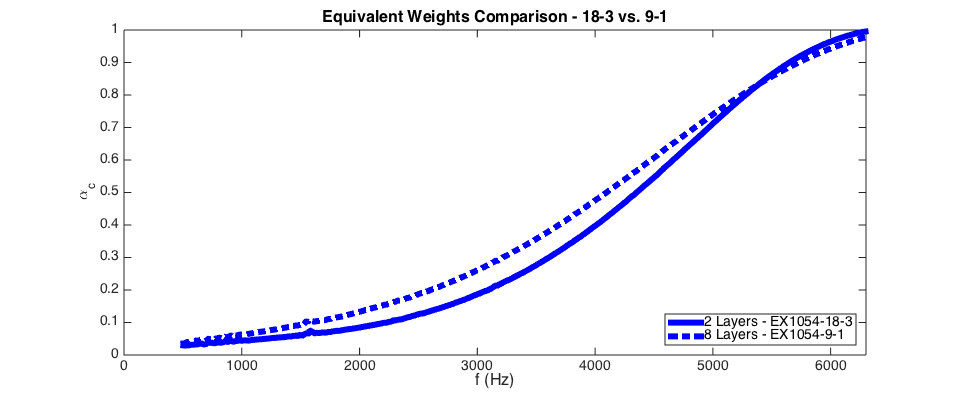
\includegraphics[width=1\textwidth]{Chapter-4/figs/AfigSOCK18-3compareSOCK9-1}
    \caption{Absorption Coefficient vs. Frequency - SOCK18-3 vs. SOCK9-1}
    \label{fig:AfigSOCK18-3compareSOCK9-1}
\end{figure}

% Absorption Coefficient - SOCK 18-3 vs. 9-9
\begin{figure}[hbtp]
    \centering
    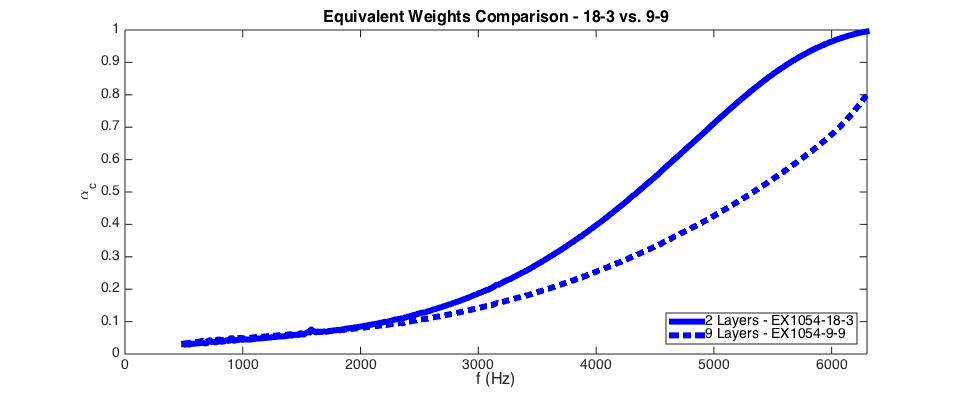
\includegraphics[width=1\textwidth]{Chapter-4/figs/AfigSOCK18-3compareSOCK9-9}
    \caption{Absorption Coefficient vs. Frequency - SOCK18-3 vs. SOCK9-9}
    \label{fig:AfigSOCK18-3compareSOCK9-9}
\end{figure}

% Absorption Coefficient - SOCK 18-4 vs. 9-3
\begin{figure}[hbtp]
    \centering
    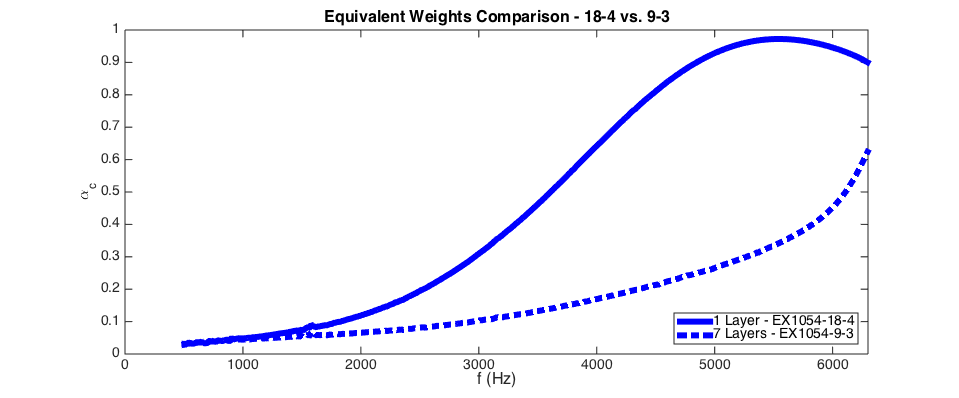
\includegraphics[width=1\textwidth]{Chapter-4/figs/AfigSOCK18-4compareSOCK9-3}
    \caption{Absorption Coefficient vs. Frequency - SOCK18-4 vs. SOCK9-3}
    \label{fig:AfigSOCK18-4compareSOCK9-3}
\end{figure}
\clearpage

\subsection{All Sock Data}
This section shows all the Sock data compiled.

% Absorption Coefficient - all compared SOCKS
\begin{figure}[hbtp]
    \centering
    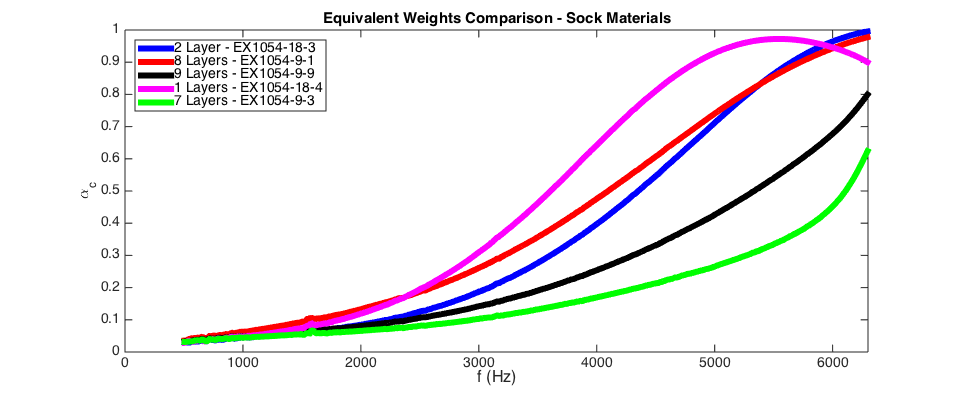
\includegraphics[width=1\textwidth]{Chapter-4/figs/AfigSOCKScompared}
    \caption{Absorption Coefficient vs. Frequency - All Compared SOCKS}
    \label{fig:AfigSOCKScompared}
\end{figure}
\clearpage

\subsection{Cellulose Acetate Sock Compared with Fiberglass}
% Absorption Coefficient - all compared SOCKS w/ Fiberglass
\begin{figure}[hbtp]
    \centering
    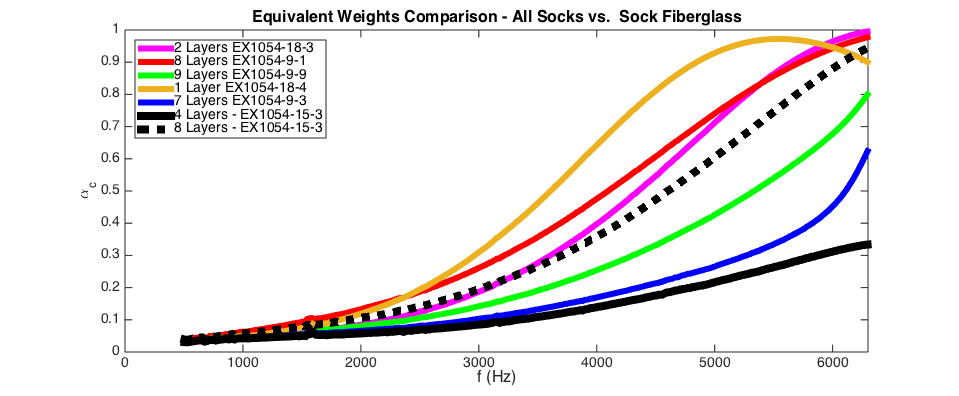
\includegraphics[width=1\textwidth]{Chapter-4/figs/AfigSOCKScomparefiberglass}
    \caption{Absorption Coefficient vs. Frequency - All Compared SOCKS with Fiberglass}
    \label{fig:AfigSOCKScomparefiberglass}
\end{figure}
\clearpage

\subsection{Filter Rods}
This section shows the filter rods as compared with Raw tow of equal mass.
% Absorption Coefficient - Raw Tow vs. Filter Rods 1.5 grams
\begin{figure}[hbtp]
    \centering
    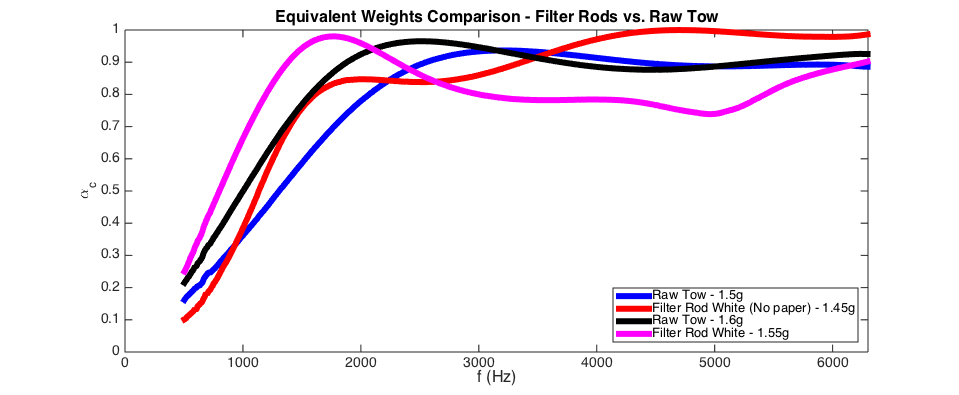
\includegraphics[width=1\textwidth]{Chapter-4/figs/Afigfilterrodscomparerawtow}
    \caption{Absorption Coefficient vs. Frequency - Raw Tow vs. Filter Rods}
    \label{fig:Afigfilterrodscomparerawtow}
\end{figure}

% Absorption Coefficient - Raw Tow vs. Filter Rods vs. Cotton
\begin{figure}[hbtp]
    \centering
    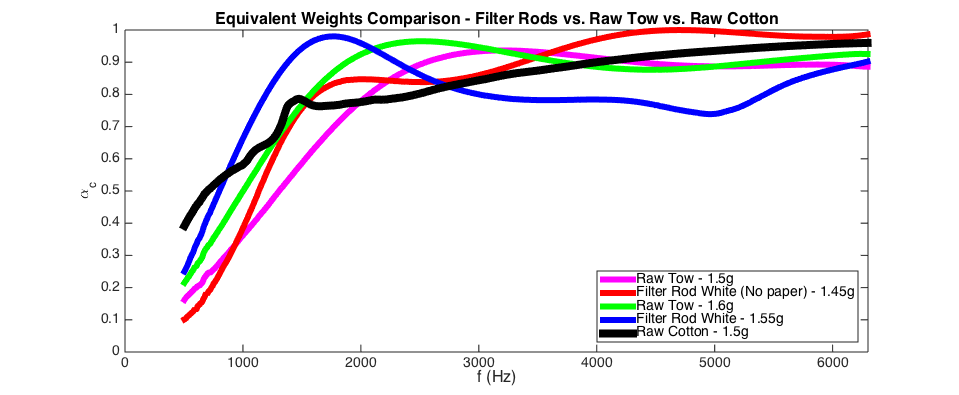
\includegraphics[width=1\textwidth]{Chapter-4/figs/Afigfilterrodscomparerawtowcomparecotton}
    \caption{Absorption Coefficient vs. Frequency - Raw Tow vs. Filter Rods vs. Cotton}
    \label{fig:Afigfilterrodscomparerawtowcomparecotton}
\end{figure}
\clearpage

\subsection{Raw Tow}
Raw Tow was analyzed with respect to Cotton of equal mass of $1.5$ grams.
% Absorption Coefficient - Raw Tow vs. Cotton 1.5 grams
\begin{figure}[hbtp]
    \centering
    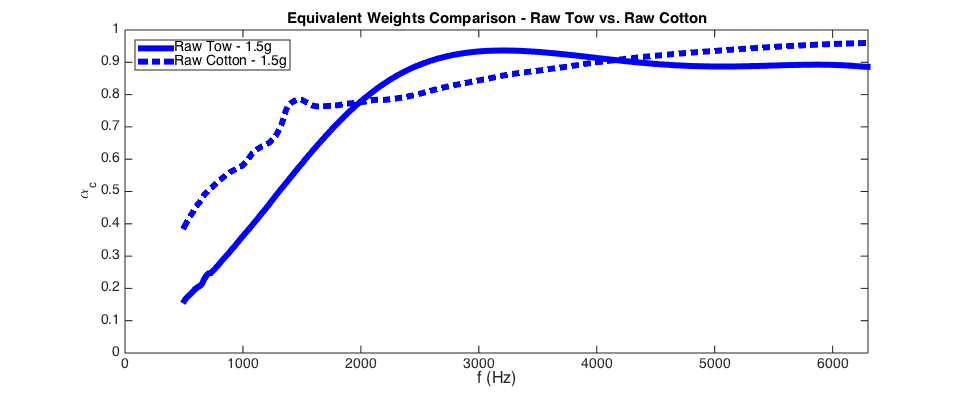
\includegraphics[width=1\textwidth]{Chapter-4/figs/Afigrawtowcomparecotton}
    \caption{Absorption Coefficient vs. Frequency - Raw Tow vs. Cotton 1.5 grams}
    \label{fig:Afigrawtowcomparecotton}
\end{figure}
